% TEMPLATE for Usenix papers, specifically to meet requirements of
%  USENIX '05
% originally a template for producing IEEE-format articles using LaTeX.
%   written by Matthew Ward, CS Department, Worcester Polytechnic Institute.
% adapted by David Beazley for his excellent SWIG paper in Proceedings,
%   Tcl 96
% turned into a smartass generic template by De Clarke, with thanks to
%   both the above pioneers
% use at your own risk.  Complaints to /dev/null.
% make it two column with no page numbering, default is 10 point

% Munged by Fred Douglis <douglis@research.att.com> 10/97 to separate
% the .sty file from the LaTeX source template, so that people can
% more easily include the .sty file into an existing document.  Also
% changed to more closely follow the style guidelines as represented
% by the Word sample file. 

% Note that since 2010, USENIX does not require endnotes. If you want
% foot of page notes, don't include the endnotes package in the 
% usepackage command, below.

% This version uses the latex2e styles, not the very ancient 2.09 stuff.
\documentclass{sig-alternate}
\usepackage{pgf}
\usepackage{listings}
\usepackage{url}
\usepackage{subfigure}
\usepackage{amsmath}
\usepackage{algorithm}
\usepackage{algorithmic}
\usepackage{flushend}

\definecolor{darkgreen}{rgb}{0,0.7,0}
\definecolor{violet}{rgb}{0.5,0.0,0.5}

\lstset{language=bash, numbers=left, numberstyle=\tiny\color{gray}, numbersep=3pt, escapeinside={\$}, basicstyle=\footnotesize\ttfamily, escapeinside={\%*}{*)}}

\newif\ifdraft
\drafttrue
%\draftfalse                                                                              
\ifdraft
\newcommand{\iannote}[1]{ {\textcolor{red}    { ***Ian:      #1 }}}
\newcommand{\katznote}[1]{ {\textcolor{blue}    { ***Dan:      #1 }}}
\newcommand{\zhaonote}[1]{{\textcolor{cyan}    { ***Zhao:      #1 }}}
\newcommand{\kylenote}[1]{{\textcolor{orange}    { ***Kyle:      #1 }}}
\newcommand{\note}[1]{ {\textcolor{red}    {\bf #1 }}}
\else
\newcommand{\iannote}[1]{}
\newcommand{\katznote}[1]{}
\newcommand{\zhaonote}[1]{}
\newcommand{\kylenote}[1]{}
\newcommand{\note}[1]{}
\fi

\conferenceinfo{SC15}{2015 Portland, OR USA}

\begin{document}

%don't want date printed

%make title bold and 14 pt font (Latex default is non-bold, 16 pt)
\title{Balancing Costs for Data Resilience}

%for single author (just remove % characters)
\author{
\begin{tabular}{cccc}
{Zhao Zhang\textsuperscript{*,\#}} & {Daniel S. Katz\textsuperscript{+}} & {Haoyuan Li\textsuperscript{*}} & {Kyle Chard\textsuperscript{+}} 
\end{tabular}
\\
\begin{tabular}{ccc}
{Ian Foster\textsuperscript{+}} & {Michael J. Franklin\textsuperscript{*,\#}} & {Ion Stoica\textsuperscript{*}}
%Name Institution
\end{tabular}
\and % use '\and' if you need 'another row' of author names
\begin{tabular}{c}
\textsuperscript{*}AMPLab, University of California, Berkeley \\
\textsuperscript{\#}Berkeley Institute for Data Science (BIDS), University of California, Berkeley \\
\textsuperscript{+}Computation Institute, University of Chicago \& Argonne National Laboratory
\end{tabular}
} 

\maketitle

\katznote{note that authors are probably not in the correct ACM format}

% Use the following at camera-ready time to suppress page numbers.
% Comment it out when you first submit the paper for review.
%\thispagestyle{empty}


\begin{abstract}
Resilience is critical for many-task applications running on large scale computing platforms in which node failures are inevitable. 
This is especially the case when using a transient in-memory file system for parallel scripting. 
The state of these scripts is stored, in practice, by the files they write, and these files are 
inherently volatile as they are not persisted to disk.
Existing systems overcome node failure by providing resilient data access either through task re-execution or file replication. 
However, applying either technique blindly can be inefficient due to 
excessive recovery or replication costs associated with the irregularity of task runtimes and I/O.
We present an adaptive method that calculates and balances backup and
recovery costs to guide resilience decisions. Our method aims to identify
at run time the best choices for a given computer system and application.
We implement this adaptive method inside the AMFORA parallel scripting framework
and evaluate its effectiveness with an image processing application, Montage.
We find that the adaptive method recovers up to 57\% faster than
do pure re-execution or replication, while introducing only 2.9\% overhead in failure-free performance on 64 compute nodes.
We also discover that, at least for this application, backup decisions are relatively insensitive to node failure rate.
%We implement the adaptive backup model inside two distributed computing framework: AMFORA and
%GraphX to enable efficient execution of parallel scripting applications and graph processing applications respectively.
%Our model enables automated selection of the `best' backup technique, providing 
%high system resilience while considering aspects such as cost and performance. Using two real world applications
%our results show that dynamic backup improves upon purely replication or lineage under failure 
%and exhibits an acceptable overhead without failure. 
\end{abstract}

\katznote{need to set categories, terms, and keywords - all below are from the template}

% A category with the (minimum) three required fields
\category{H.4}{Information Systems Applications}{Miscellaneous}
%A category including the fourth, optional field follows...
\category{D.2.8}{Software Engineering}{Metrics}[complexity measures, performance measures]

\terms{Theory}

\keywords{ACM proceedings, \LaTeX, text tagging}
\section{Introduction}
%\zhaonote{the overall tone of this paper is about unreliable distributed computing platforms, I will make it more supercomputer, and declare we are emulating a supercomputer with Amazon EC2.}
%\{test}
Distributed computing applications have long strived to %provide system resilience in the presence of 
be resilient to 
unreliable computing nodes. As applications scale to thousands and tens of thousands of 
compute nodes, the likelihood of a single node failing during execution increases proportionally~\cite{gfs2003, exaroadmap2011}. 
%\zhaonote{below is new text to shape the platform as a supercomputer, and declare what we are doing, and the goals}
We seek to build a resilient parallel scripting framework to enable many-task applications on computing platforms such as supercomputers. We model such platforms as an execution 
environment comprised of multiple nodes, each of which can independently store data. Nodes are unreliable; if a node fails, the data that it stores is lost. 
Our resilience mechanisms aim to enable continued (and uninterrupted) application execution in the presence of node failures. 
Importantly, we aim to minimize overhead in the failure-free case while providing rapid recovery in the presence of a failure.

%\kylenote{Could delete the following paragraph?} \katznote{I think it's needed}
%\zhaonote{yes, the short and many task abstraction is the reason why we can give up on the checkpointing method.}
In parallel computing, much previous research has focused on checkpointing process states to stable storage in order to tolerate failures, assuming the computation is a long-running parallel task that must be periodically checkpointed. 
Upon failure, the processes halt execution, reach a consensus, roll back to the checkpoint, and then resume execution. 


In the MapReduce~\cite{mapreduce-04} and Many Task Computing~\cite{raicu08} models,
the abstraction of a single, long-running task is replaced by many, often short-lived tasks 
that are linked by producer-consumer data sharing relationships.
Many scientific applications are also naturally composed of numerous small tasks~\cite{FALKON-SC-08}. 
This short task abstraction removes the need for coordinated checkpointing: we can think of tasks of atomic units that either execute to completion
or fail, and rethink system resilience in terms of ensuring the availability of the data that flows between tasks.
It then becomes possible to recover from node failure simply by recreating data located on the failed node. 
If we have preserved either metadata describing how to re-execute a task (a {\em lineage} backup) or the data itself (a {\em replication} backup),
we can achieve this by 1) re-executing the task(s) that produced the missing data or 2) accessing copies of that data located on other nodes, respectively.
Meanwhile, all other tasks can continue running as they are not affected by the failure.

The two backup and recovery methods described above have been employed in various systems. For example,
the Spark~\cite{RDD2012} and BAD-FS~\cite{badfs2004} systems re-execute tasks following node failure,
while RAID 1~\cite{raid1988} and the Hadoop Distributed File System (HDFS)~\cite{HDFS} replicate each file (at the block level) a configurable number of times to preserve data access following node failure.
However, irregular execution times, data sizes, and data dependencies can cause problems for each approach when applied to many-task applications. 
Universal application of the re-execution method can result in excessive recovery costs, since a failure can 
require restarting deep in the lineage graph.
On the other hand, ubiquitous application of replication method may result in excessive overheads when failures are rare, due to data copying and storage costs.
Thus, we present here a new configurable adaptive method that dynamically chooses between these two methods,
based on online, model-driven estimates of backup and recovery costs. We integrate this adaptive method into
AMFORA~\cite{AME, AMFS2013},
a parallel scripting framework for scientific computing, and evaluate its performance in the context of a large many task scientific application, Montage~\cite{montage2, montage1}. 
Our experiments show that when emulating a supercomputer using 64 m3.large Amazon EC2 instances, the adaptive model recovers up to 57\% faster than a purely re-execution or replication approach, and introduces only 2.9\% of failure-free overhead. %when compared to no backups.
%The experiment of PageRank of GraphX on the Twitter dataset shows \zhaonote{need to update the number}

The contributions of this work are the use of a general adaptive mathematical model for making dynamic resilience %\zhaonote{I prefer resilience, as we actually make backup decisions that can make recovery fast.} %backup\kylenote{is backup the right word here? maybe recovery, resilience or replication?}
decisions and evaluation of this model in a practical setting.
The model is applicable to a broad range of applications running on clouds, clusters, and supercomputers. We also show that node failure rate is irrelevant to backup choice decision in practice.

The rest of paper is organized as follows:
Section~\ref{sec:background} briefly introduces Montage and AMFORA, including AMFORA's architecture, programming model and data management.
Section~\ref{sec:Model} introduces the task abstraction, the analytical model, and the dynamic replication algorithm. 
Section~\ref{sec:Impl} describes the changes made to AMFORA 
to implement the resilience model, including solutions to additional technical problems. 
Section~\ref{sec:Perf} presents and analyzes the performance of the resilience model.  
Section~\ref{sec:Related} surveys previous work in system resilience.
Finally, Section~\ref{sec:Con} summarizes the work and envisions future research.

\section{Background}
\label{sec:background}
In this section, we briefly introduce the Montage application and AMFORA's programming, data management, and task management models.

\subsection{Montage}
Montage is an astronomy image processing application that assembles large mosaics from multiple small images obtained from telescopes, while preserving the amount and position of the energy. 
Figure~\ref{fig:montage-flow} shows the data flow of montage application.
Table~\ref{tb:Montage} explains the application stage by stage.

\begin{table}[h]
    \caption{Montage tasks}
   \begin{small}
    \begin{tabular}{ | p{1.8cm} | p{5.7cm} |}
    \hline
    Stage & Description  \\ \hline \hline
    mProject &  reads image files and writes reprojected images\\ \hline
    mImgtbl &  takes the one line from mProject output, and concats them into one file\\ \hline
    mOverlaps &  analyzes the image table, produces a metadata table describing which images overlap along with a task list of {\tt mDiffFit} tasks (one for each pair of overlapping images) \\ \hline
    mDiffFit &  inputs two overlapping output files from {\tt mProject}, fits a plane to the overlap region \\ \hline
    mConcatFit &  gathers all output data from the previous stage (coefficients of the planes), and summarizes them into one file \\ \hline
    mBgModel &  analyses the metadata from {\tt mImgtbl} and the data from {\tt mConcatFit}, creating a set of background rectification coefficients for each image, then generates a {\tt mBackground} task list \\ \hline
    mBackground &  applies coefficients to the reprojected images\\ \hline
    mAdd &  reads output files from {\tt mBackground}, and writes an aggregated mosaic file \\ \hline
    \end{tabular}
    \end{small}
      \label{tb:Montage}
\end{table}

\begin{figure}[h]
\begin{center}
    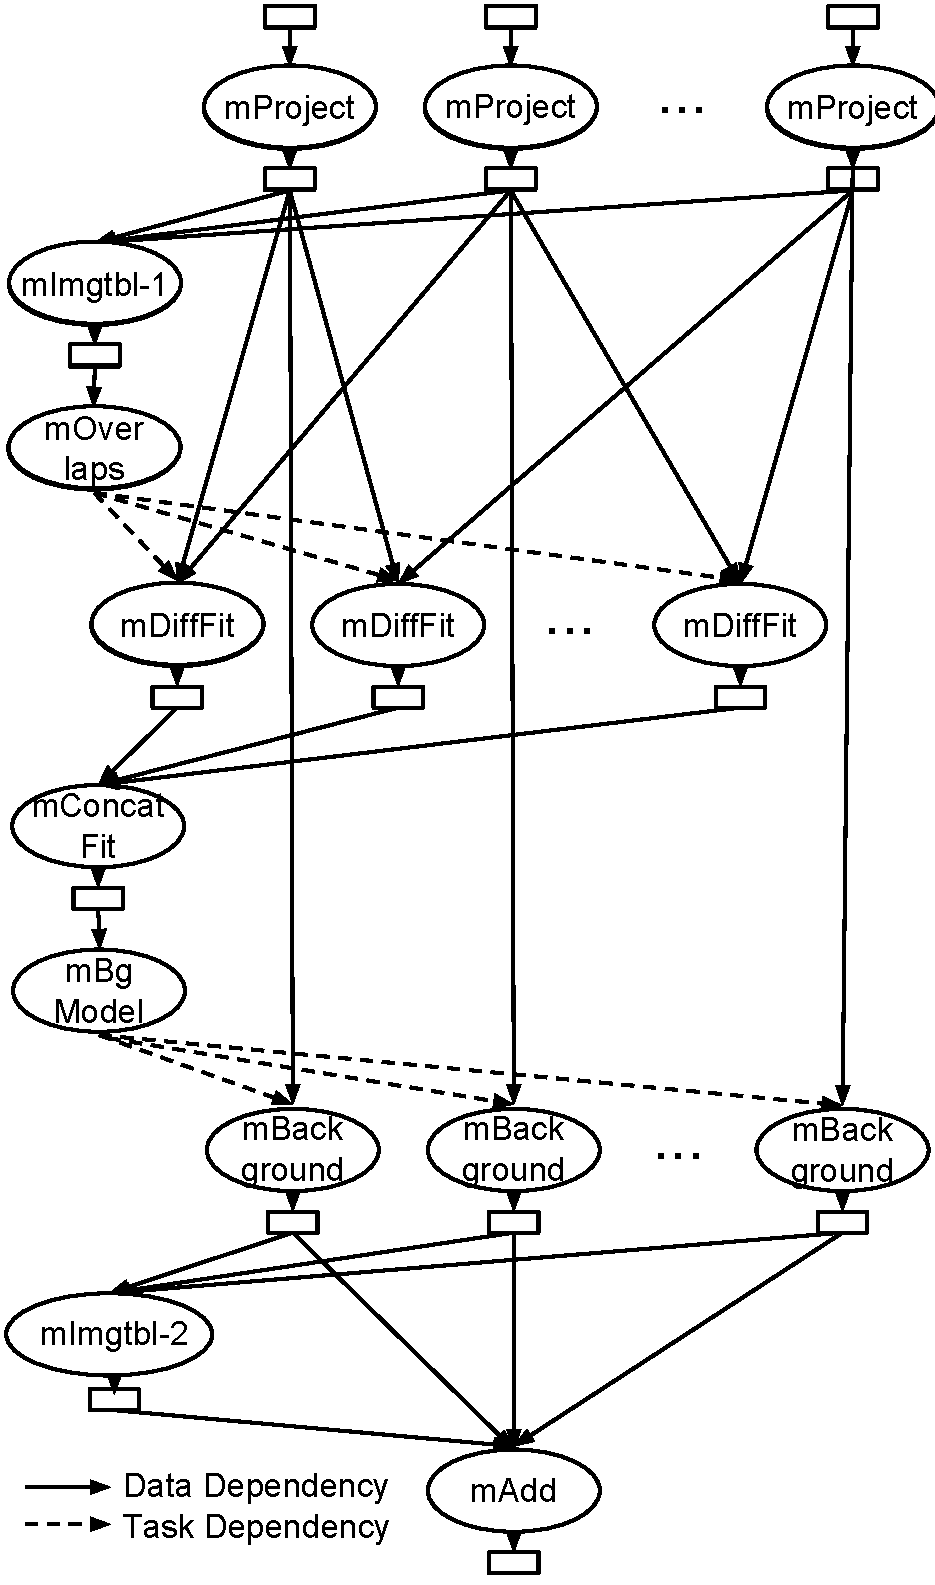
\includegraphics[width=68mm]{pictures/montage}
\caption {Montage data flow. Ovals represent tasks and boxes represent files. Solid lines show data dependencies, dashed lines show task dependencies.
    \label{fig:montage-flow}
}
\end{center}
\end{figure}



\subsection{AMFORA}

AMFORA is a POSIX-compatible parallel scripting framework that allows users to run (unmodified script-based) 
programs in parallel with data stored in the distributed RAM-based AMFORA File System.  
AMFORA provides a simple programming interface to its task and data management capabilities.
In essence, the programmer specifies many task computations in terms of operations performed on files,
with operations on directories serving to specify collective transformations on many files.

\subsection{AMFORA Programming Model}
AMFORA script code for the first two stages of the Montage application is shown in Listing~\ref{lst:Montage}.
\begin{lstlisting}[label=lst:Montage, caption=Parallel Script for Montage, xleftmargin=2.5ex]
#!/bin/bash

#mProjectPP
#for each file in rawdir/ we run a  
#mProject task with it as input file   
#and produces an output file stored  
#in tempdir/

#Queue is the API to push a task into 
#the queue
#Execute is the API to run the queued  
#tasks in parallel

mkdir tempdir/
for file in `ls rawdir/`
do
  %*\texttt{\textbf{Queue}}*) mProject rawdir/${file} \
    tempdir/hdu_${file}
done
%*\texttt{\textbf{Execute}}*) 

#Gather API moves all files stored in 
#tempdir/ to a single node

#Then the mImgtbl task is launched to
#processes the files and write outputs 
#to images.tbl
%*\texttt{\textbf{Gather}}*)  tempdir/
mImgtbl tempdir/ images.tbl 	    
\end{lstlisting}

Lines 14--19 enqueue tasks; line 20 dispatches all queued tasks  
to available compute nodes for execution. Line 28 is a simple example of AMFORA collective data movement:
it moves all files in the {\tt tempdir/} directory from multiple nodes to a single node using a minimum-spanning tree algorithm.
AMFORA supports multicast, gather, scatter, allgather, and shuffle (alltoall) data flows.

\subsection{AMFORA Task and Data Management}
Tasks are launched by the AMFORA Execution Engine, which also monitors their execution and collects runtime information
that is subsequently used as input to the backup decision process.
Information collected includes per-task queue time, start time, and end time, plus file usage (input or output) based on observations
of runtime state mutations.

The AMFORA File System manages three types of data: directory metadata, file metadata, and file data.
Every compute node in an AMFORA system is both a metadata server and an I/O server. 
The file system implements multi-reader single-writer consistency: a file can be read multiple times from multiple processes but can only be written by a single process once. Once a file is released (a POSIX primitive) from writing, it cannot be modified further. 

All directory metadata is managed synchronously across all compute nodes. This synchronization does not represent
a significant bottleneck as the creation 
and mutation of directories is rare in many-task applications~\cite{MTC-Bluewaters}.
File metadata is mapped across compute nodes via consistent hashing. 
The hash function assumes a ring topology composed of all compute nodes and, for each file,
uses the hash of the file path to find the node that stores that file's metadata.
File data is primarily stored where it is produced, so as to avoid remote writes. AMFORA does not
support the partitioning or distribution of files across multiple nodes. While a limitation and 
a potential area for future work, this restriction does not represent a significant limitation in practice, as file sizes are generally
small in many-task applications~\cite{MTC-Bluewaters}. 

%\subsection{AMFORA Task Management}

%\subsection{GraphX}
%text



\section{Adaptive Backup and Recovery Model}
\label{sec:Model}
%\kylenote{Should this section be called adaptive backup and recovery model?}

Our resilience method builds on an analytical model that relates the costs of backup and recovery to system parameters
such as communication cost and failure rate.
Here we explain this model in detail and present the algorithm that we use to make dynamic resilience decisions. 

In general, we view a task as a function $t$ that takes $n$ input files and produces $m$ output files:
\begin{equation}
y_{1}, \ldots, y_{m} = t(x_{1}, \ldots, x_{n})
\end{equation}
%
Table~\ref{tab:modelterms} defines these and other terms used in subsequent discussion.

%\kylenote{Could these assumptions come later?} \katznote{perhaps could be moved to the start of Section 3}
We assume the network that connects nodes has a uniform bandwidth and latency to simplify the discussion; we later show that this works reasonably well in practice. 
In the case of node failure, we assume that the data stored in that node is not accessible, which is true for the case of a supercomputer where there is no local disk.
%\zhaonote{add more words to previous sentence to make it supercomputer} 
%\katznote{future supercomputers, as well as some past ones, have had local disk} 
%\zhaonote{shall I say ``in the case of there is no local disk'', if there is local disk, someone may challenge why do not use asynchronous replication to disk since disk failure is rare?}
We assume lineage information gathering and data replication are synchronous. To simplify the discussion, we also assume that all nodes share a common, consistent failure rate and failures are uncorrelated. However, we later show that the failure has little impact on the adaptive backup model in Section~\ref{sec:Perf:Failure}. 


\begin{table}
\centering
\caption{Resiliency model terms.}
\label{tab:modelterms}
\begin{tabular}{|p{1cm}|p{6.25cm}|} \hline
Term & Meaning \\ \hline
{$P$} 					& rate of failure, i.e., $\frac{1}{MTTF}$ \\
{$timeout$} 					& time required to switch from one replica of a data item to another, e.g., due to waiting for timeout \\
{$T$}					& time to solution of a task without failures\\
{$r$} 					& number of metadata and file replicas \\
{\em B} 				& network bandwidth (assumed uniform) \\
{$U_{repl}(x)$} &  time to backup data item {\em x} using replication \\
{$U_{line}(x)$} &  time to backup data item {\em x} using lineage \\
{$E_{repl}(x)$} &   time to recover data item {\em x} using replication \\
{$E_{line}(x)$} &   time to recover data item {\em x} using lineage \\
{$x_i$} 				& the $i$th input file of a task \\
{$y$}				& an output file of a task \\
{$|y|$}				& size of file $y$ \\
{$|M_{y}|$}		& size of file $y$'s metadata including the lineage information that can reproduce $y$\\
\hline\end{tabular}
\end{table}


\subsection{Backup Cost}
%\kylenote{we seem to flip flop between calling it re-execution or lineage. I vote for re-execution and talk about that based on lineage metadata as you do here} \katznote{agreed}
A file can be recovered either by retrieving a replica or through re-execution based on its lineage metadata.  To create $r$ replicas of a file or its lineage metadata, $r-1$ additional copies are needed.  The time required to synchronously create the $r-1$ replicas of a file $y$ to memory is as follows:

\begin{equation}
U_{repl}(y) = \frac{|y|}{B} (r-1)
\end{equation}

Similarly, the time required to synchronously replicate the lineage metadata of a file $y$ $r-1$ times is as follows.
\begin{equation}
U_{line}(y) = \frac{|M_{y}|}{B} (r-1)
\end{equation}

\subsection{Expected Recovery Cost}

We can now estimate the expected recovery time via replication or re-execution, given the assumptions above.
%Given an unreliable environment in which compute nodes fail with rate $P$, 
%a network with uniform bandwidth $B$, we can estimate the expected recovery time.

\subsubsection{Expected Replication Recovery Cost}
If a file $y$ is replicated on multiple nodes,
its expected replication recovery cost $E_{repl}(y)$ can be evaluated as the sum
of the expected recovery cost in the following cases:

\noindent ~~~~ The first replica is available: $(1-P)\frac{|y|}{B}$

\noindent ~~~~ The second replica is available but not the first:\\

\vspace{-2ex}

~~~~~ $P(1-P)\left(\frac{|y|}{B}+timeout\right)$

\noindent ~~~~ etc.

\noindent where $timeout$ is the time for the system to switch from one replica to another.

We add these items and transform the equation to:
\begin{equation}
E_{repl}(y) = \frac{|y|}{B}\left(1-P^r\right) + \left(\frac{P-P^r}{1-P}-(r-1)P^r\right)timeout
\end{equation}

As $P^r$ is small, we can replace it with $0$ to obtain the following closed form approximation:

\begin{equation}
E_{repl}(y) \approx \frac{|y|}{B}+\frac{P}{1-P}timeout
\label{EQ:spatial}
\end{equation}
Equation~\ref{EQ:spatial} defines the replication recovery cost for an output file $y$ to be approximately 
equal to the time required to transfer the file plus the time required to switch to the replica
in the case of failure, where the likelihood of needing to use the replica is based on the rate of failure $P$
Thus, when there is no failure, the cost of replication is simply the cost of creating the replicas

\subsubsection{Expected Re-execution Recovery Cost}
The recovery time via re-execution is dependent on both the time to re-execute the task as well
as the time to recover the required input files of that task. 
A task $t_i$ has $n$ input files. Assume that those input files are located on $n$ other nodes.
The probability that a node is available is $(1-P)$. The probability that all $n$ nodes are available is $(1-P)^n$.
The expected recovery time through re-execution is
$(1-P)^nT$. 
If there are one, two, or more failed nodes, the expected recovery time through re-execution is:

\noindent ~~~~ One failure:
%
${n \choose 1}P(1-P)^{n-1}(T+E(x_i))$

\noindent ~~~~ Two failures:

~~~~~ ${n \choose 2}P^2(1-P)^{n-2}(T+E(x_i)+E(x_j))$

\noindent ~~~~ etc.

\noindent where ${E(x_i)}$ refers to the recovery cost of item ${x_i}$ via the technique with which file ${x_i}$ is backed up. 


Adding these items gives the following closed form for the expected re-execution recovery cost:

\begin{equation}
E_{reex}(y) = T+P\sum_{i=1}^{n}E(x_i)
\label{EQ:temporal}
\end{equation}

Equation~\ref{EQ:temporal} defines the re-execution recovery cost for an output file $y$ to be
equal to the time to re-execute the task $T$ plus the sum of the time required to recover all of $T$'s
input files. Here, the only overhead (in the case without failure) is related to 
the cost of updating file metadata with the information needed to re-execute the task.

\subsubsection{Combining Backup and Recovery Cost}
To simplify our discussion, we assume a task writes its output files first to local cache, then backs up the files synchronously with the specified technique. Thus the total time taken by a task is the sum of three parts:
{\bf T}: task execution time, including computation and I/O cost,
{\bf U}: time to backup the output file or lineage metadata, %\kylenote{Would it be clearer to say backup the output file or lineage metadata?}\zhaonote{fixed}
and {\bf E}: expected cost to recover the output file. %\kylenote{Is the expected cost to recover the output part of the time?}

To take both the backup cost and expected recovery cost into account, we use a linear combination of {\bf U} and {\bf E}, which we call % as the indicator score\iannote{A phrase that is unfamiliar to me.} 
Score $S$, shown in Equation~\ref{EQ:combined}:
\begin{equation}
S=\alpha*U+(1-\alpha)*E
\label{EQ:combined}
\end{equation}
%
For every output file, we evaluate the total cost with both re-execution and replication as the backup choice, and use the one with the lower total cost.
%\kylenote{This first sentence seems wrong, we choose the method based on the ratio? If recovery cost is favored we could end up using the backup choice with greater cost?} 
%\zhaonote{Yes, that is correct. We compute $S_{replication}$ and $S_{re-execution}$, and choose the method with lower score. Let's say if a user favors recovery cost, it may end up in the situation where the failure-free time-to-solution is longer. But it is ok, all we guarantee in that case is that if there is a failure, we recover faster. The model is actually a tradeoff between failure-free performance and failure-present performance.}
The term $\alpha$ in Equation~\ref{EQ:combined} is a weight, which the user can set to between 0 and 1. 
 If the user's optimization goal is backup cost, users can set $\alpha$ close to 1.
That means that execution will optimize the backup cost over recovery cost. 
During execution, the system will always select the backup method with lower backup cost, thus minimizing the failure-free overhead.
%\zhaonote{add one sentence to explain what it means for application with the weight $\alpha$}
In contrast, if the user's optimization goal is recovery cost, $\alpha$ should be set close to 0. 
The system make backup decisions to optimize the expected recovery cost since the chance of failure is high. 
%So the system will always prefer to optimize the performance with the presence of failures.
%\zhaonote{add one sentence to explain what it means for application with the weight $\alpha$} 
%\katznote{I don't understand the previous sentence}
%\zhaonote{I removed that sentence, it says the something as its previous.}
Section~\ref{sec:Perf:Weight} quantitatively evaluates the impact of optimization weight on adaptive backup decision making. 

\subsubsection{Discussion}
%\kylenote{I'm not sure if this section adds a lot, I'm not sure if the discussion is based on what you think? or are we forward referencing results? I would vote to remove (although the picture is nice).}
%\katznote{I think this makes sense to keep - it explores the equations we just presented.}
We next discuss how task and system parameters impact the choice of backup method.
The four example tasks in Figure~\ref{fig:taxonomy} vary in their computation time, I/O size, and number of input files. If we control the comparison by varying only one factor, we can observe some trends about backup decisions.
An output file produced by a long-running task will tend to be backed up by replication because the cost of regenerating the file via task re-execution is likely to be large.
%\iannote{It is unclear from the text whether the following are qualitative statements based on your intuition, or based on simulations.}
%\iannote{Do you not assume that there is just one output file per task?} 
%\iannote{I realize now something that is bothering me. You seem to alternate between a perspective based on files and a perspective based on tasks. I think the text will be clearer if you choose one. Let's say it is files. Then this sentence would be ``An output file produced by a longer-running task will tend to be backed up by replication." This sentence (and the other sentences in this section) would be clearer if we added some explanatory words, such as ``because the cost of regenerating the file by re-executing the task will be large."}\zhaonote{I see, fixed}
A large output file is more likely to be backed up through re-execution, since replication may be time consuming.
A file that depends on more input files has a higher probability to be backed up through replication, as reading many input files (required to re-execute the task) may consume a significant period time.
%
System bandwidth also factors into the choice of backup method:
higher bandwidth improves replication performance more significantly than re-execution, and thus, other things being equal, the same file is more likely to be backed up through replication on a higher-bandwidth system.

\begin{figure}[ht]
	\begin{center}
		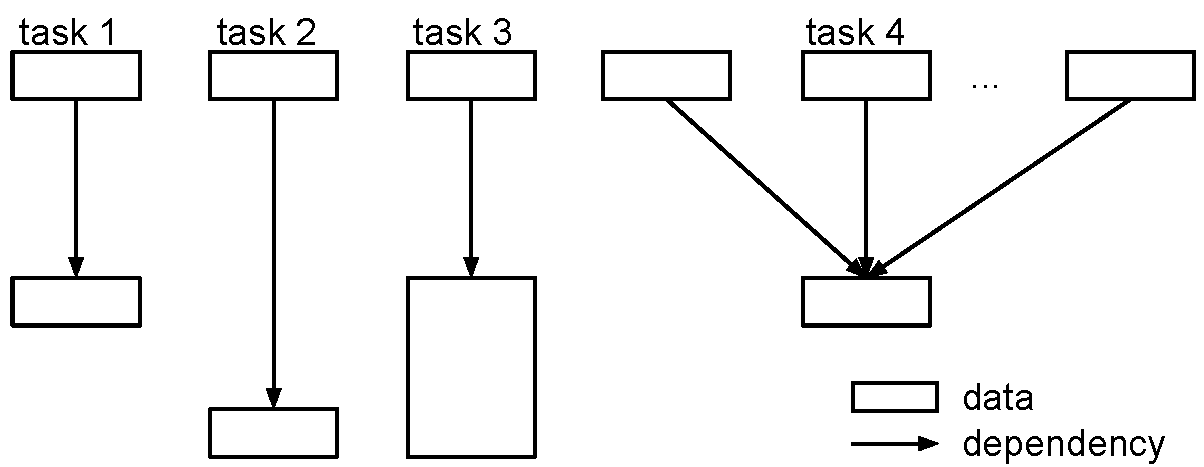
\includegraphics[width=75mm]{pictures/task-taxonomy}
		\caption{Example tasks in a three dimensional space of computation time, I/O size, and number of input files. Rectangles are data, rectangle area is proportional to data size, arrows are data flows, and the length of arrows indicates task computation time.
		\label{fig:taxonomy}}
  	\end{center}
\end{figure}


\section{Implementation}
\label{sec:Impl}
To integrate the adaptive backup model into the AMFORA framework, we implemented two backup primitives: replicate() and re-execute(). The {\em replicate()} primitive creates a configurable number of replicas for a file on peer nodes. The {\em re-execute()} primitive records a file's lineage (i.e., the command line used to produce it) in the file's metadata. Also recorded in the file metadata are the file's host address and expected recovery costs via both methods.
The execution engine captures task runtime information such as time-to-solution and I/O size. We also require that it
identify which parameters in the command line are input files and which are output files.

\begin{figure}[ht]
	\begin{center}
		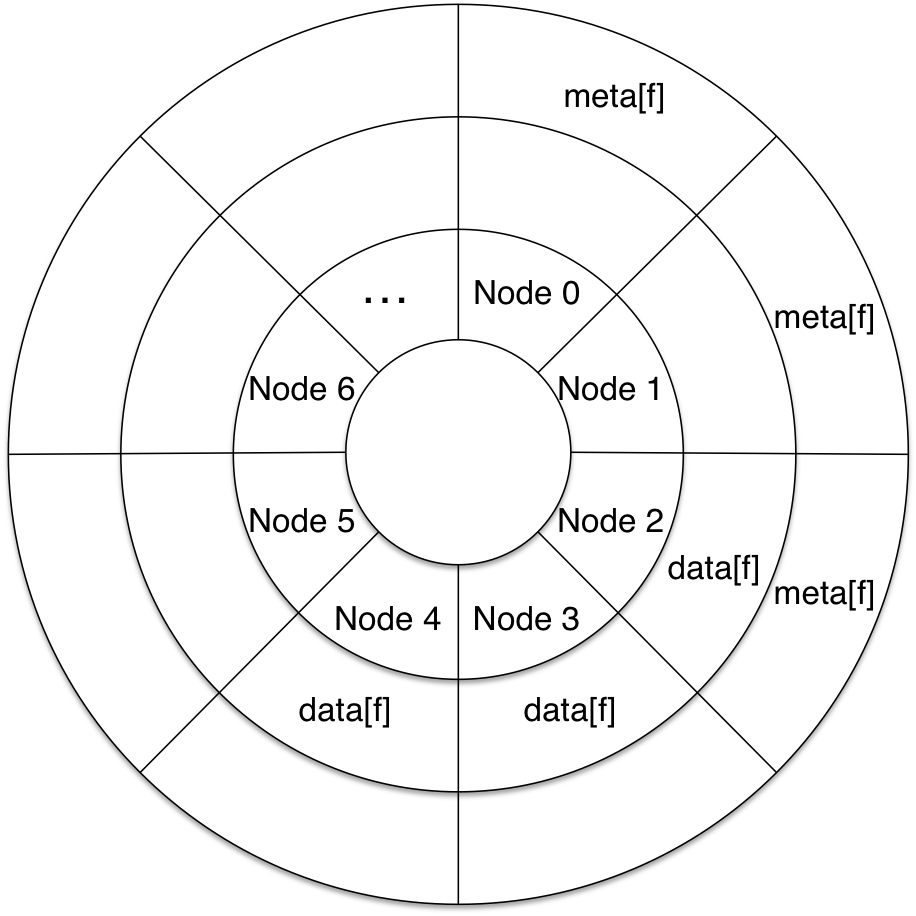
\includegraphics[width=68mm]{pictures/datalayout}
		\caption{A data layout example with three-way replication. Node 2 produces file f, and Node 0 hosts f's
		metadata. Node 0 is chosen to host f's metadata by hashing f's file path. The actual data of f is replicated to Nodes 3 and 4, and the metadata is replicated
		to Nodes 1 and 2.
		\label{fig:datalayout}}
  	\end{center}
\end{figure}

Both files and their associated metadata are copied to peer nodes a configurable number of times.
File replicas are placed on nodes directly adjacent to the file hosting node in the ring topology.
Similarly, metadata are copied to nodes adjacent to the metadata hosting node.
Figure~\ref{fig:datalayout} shows an example data layout in which three copies each have been
created for both the data ({\tt data[f]}) and metadata ({\tt meta[f]}) of a file {\tt f}.
To access file data or metadata, a client applies a consistent hash function, with the file path and node list as input, to determine the node that hosts the file data or metadata. If access to that node fails, it can switch to the next copy until the required item is returned. (The client can infer locations of copies beyond the first based on global topology information.

Recovery of a file for which no copy exists requires access to the file's lineage metadata.
This metadata is retrieved and the computation that it describes is examined to
determine whether the input file(s) needed to create that file are present. If they are not, the process is repeated for each input file.
The resulting directed acyclic graph of tasks is then executed.

Our implementation is also responsible for synthesizing lineage metadata and for
maintaining the database of file sizes and task execution times that is
used to guide backup decisions. To this end, the execution engine tracks modifications to all
local metadata and data
in order to gather task execution times and file usage patterns.
This information allows each compute node to make individual backup decisions for each new
file that is generated.



\section{Performance Evaluation}
\label{sec:Perf}
We evaluate the adaptive method by emulating a supercomputer environment with an Amazon EC2 cluster of 64 m3.large instances, each equipped with 2 Intel Xeon E5-2670 vCPUs and 7.5~GB memory.  (Note: we use Amazon as a cluster because that there are technical barriers to performing our evaluation on many supercomputers: Cray systems do not allow users to use FUSE on compute nodes, and BG/Q systems do not have a full Linux kernel.)
%\zhaonote{rewrite the previous sentence to make it supercomputer} 
%\katznote{not sure this is really helpful - reviewers might ask why not just use 64 nodes of a real supercomputer}
%\zhaonote{There is some technical barrier for running AMFORA on supercomputers after BG/P is decommissioned. The NERSC Edison machine does not allow users to use FUSE on compute nodes and so do other Cray ones. BG/Q does not have a full linux kernel yet.}

The Montage test case is a 3x3 degree image mosaic of 2MASS data centered at Galaxy m101. 
The application has 369 initial input files (raw images) and one final output file (mosaic). 
The application has nine stages (mImgtbl is executed twice). 
The mProject, mDiffFit, and mBackground stages have multiple tasks. 
The mImgtbl, mConcatFit, and mAdd stages have a single task but a large number of input files. 
Table~\ref{tb:montage-stats} summarizes the basic statistics of each stage of the Montage test case.

The Montage application can also be viewed as eight independent applications that each have different computation and I/O properties. 
The nine stages spans a wide space of many-task applications across dimensions of relative data/computation intensiveness and parallelism (single task stage and distributed stage).
%\zhaonote{add previous paragraph to argue the coverage of Montage}

\begin{table*}[ht]
\begin{center}
    \caption{Number of tasks, inputs, and outputs, and input and output size, for each Montage stage}
    \begin{scriptsize}
    \begin{tabular}{ | p{1.6cm} | p{1cm} | p{1.1cm} | p{1.35cm} | p{1.1cm} | p{1.35cm} | p{1.3cm} | p{1.55cm} | p{3.3cm} |}
    \hline
    Stage & \# Tasks & \# \mbox{Inputs} & \# \mbox{Outputs} & \# \mbox{Inputs} per Task & \# \mbox{Outputs} per Task & Max \mbox{Input} Size (MB) & Max \mbox{Output} Size (MB) & Input Dependency\\ \hline \hline
	mProject & 369 & 369 & 738 & 1 & 2 & 2.1 & 4.2 & filesystem \\ \hline
	mImgtbl-1 & 1 & 369 & 1 & 369 & 1 & 4.2 & 0.97 & mProject\\ \hline
	mOverlaps & 1 & 1 & 1 & 1 & 1 & 0.97 & 0.13 & mImgtbl\\ \hline
	mDiffFit & 1065 & 369 & 2030 & 2 & 2 & 4.2 & 0.5 & mProject\\ \hline
	mConcatFit & 1 & 1065 & 1 & 1065 & 1 & 0.5 & 0.5 & mDiffFit\\ \hline
	mBgModel & 1 & 2 & 1 & 2 & 1 & 0.5 & 0.5 & mImgtbl, mConcatFit\\ \hline
	mBackground & 369 & 369 & 369 & 1 & 1 & 4.2 & 4.2 & mProject\\ \hline
	mImgtbl-2 & 1 & 369 & 1 & 369 & 1 & 4.2 & 0.97 & mBackground\\ \hline
	mAdd  & 1 & 369 & 1 & 369 & 1 & 4.2 & 1200 & mImgtbl-2, mBackground\\ \hline
    \end{tabular}
    \end{scriptsize}
    \label{tb:montage-stats}
\end{center}   
\end{table*} 

\begin{figure*}[ht]
	\begin{center}
		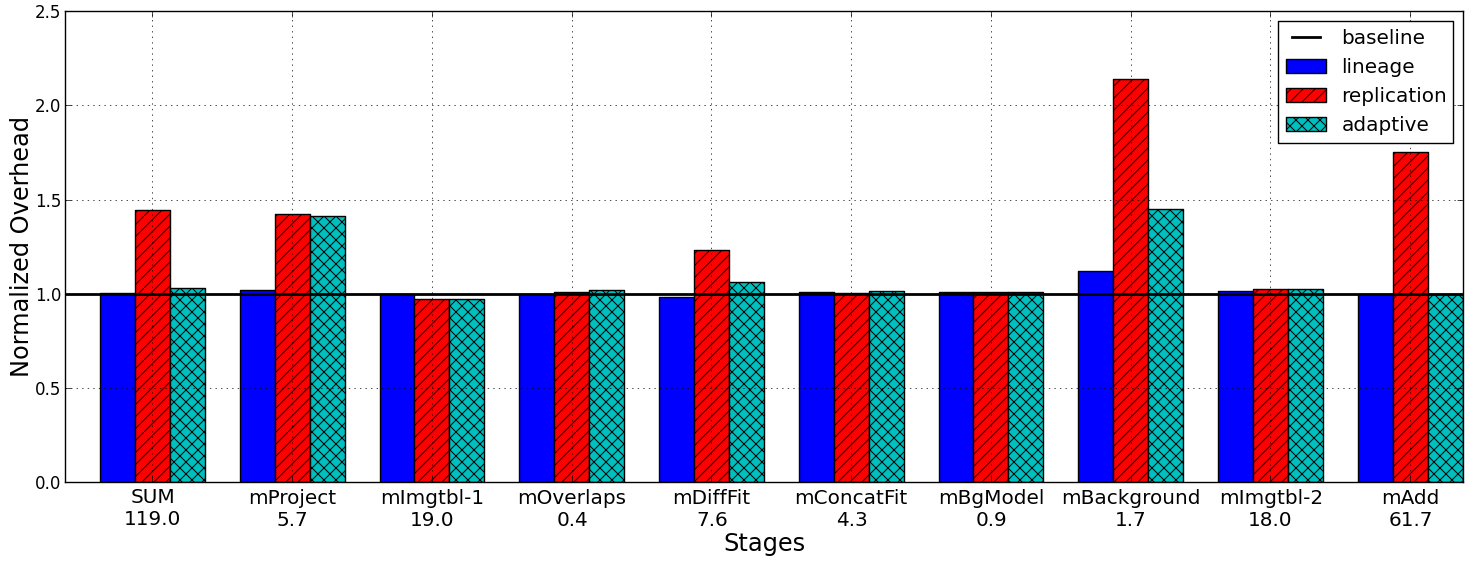
\includegraphics[width=160mm]{pictures/no-failure.png}
		\vspace{-10pt}
		\caption{Montage performance comparison of lineage backup, replication backup, and adaptive backup
		methods without node failures during execution, shown as ratios between the time-to-solution 
		of each resilience method against the no-resilience time-to-solution. Bars above the line indicates performance degradation,
		and bars below the line indicates performance improvements. The numbers underneath the stage labels are the baseline time-to-solution measured in seconds for overall application and each stage.
		\label{fig:montage}}
  	\end{center}
\end{figure*}

In our recovery cost model we specify a network bandwidth ($B$) of 20~MB/s, which was measured in the EC2 cluster. The optimization weight ($\alpha$) is set to 0.5, which means backup cost and expected recovery cost are treated equally. Since the overall application runs in 200 seconds, we set the rate of failure ($P$) as $\frac{1}{12800}$ (one fault per run).


\subsection{Failure-free Backup Overhead}
We first run a set of experiments to measure costs incurred by our adaptive method in the absence of failure.
We run the nine stages
of the Montage application on our target platform using four different system configurations: no-resilience, re-execution backup,
replication backup (two replicas per file), and adaptive backup.
Figure~\ref{fig:montage} shows, for each of the latter three cases, the resilience overhead expressed as
the ratio between its execution time and the no-resilience time.

We see that in the failure-free case, the overhead incurred by the re-execution approach is small (just 0.6\%),
as the only substantial additional work is that of inserting the generating task (lineage) information into the file metadata.
The replication method introduces a larger overall overhead of 44.0\%, due to the need to replicate the output files
to two other nodes.

At the individual Montage stage level, the re-execution method incurs less overhead than the replication method in all stages except mImgtbl-1,
which is just one task that reads all output files from mProject.
With the replication method, mImgtbl-1 takes advantage of fact that some of the additional replicas of the mProject output files are local and don't need to be transferred.
%\kylenote{I dont understand what you mean by take advantage of replica locality?}
%\zhaonote{Let's say mProject has 369 output files, if there is no replication, each node has about 6 files (64 nodes). By replicating the file two additional times, each node will have 18 files. So mImgtbl-1 will have 18 out of 369 files in the local this. Thus it can run faster.}
In the mBackground stages, the re-execution method's overhead is significant (12.1\%), because this stage involves many
parallel, short tasks; the many concurrent metadata updates that result can introduce contention on the nodes that host the metadata.
In contrast, the mProject, mDiffFit, mBackground, and mAdd stages all incur significant overhead when using replication, because they each produce many and/or large output files.
For example, mDiffFit has over 2000 output files and mAdd has one task that writes one 1.2~GB output file.

The adaptive method incurs an overall overhead of 2.9\%, which is in between the overheads from re-execution and replication.
For the mImgtbl-1, mOverlaps, mConcatFit, mBgModel, mImtbl-2 and mAdd stages, the adaptive
method uses lineage backup.
mDIffFit runs faster with the adaptive method than with replication, since its input files (outputs of mProjectPP) are backed up with replication.
The mBackground stage runs in a time that is between that of the re-execution and replication cases partially because the input files
were replicated, and the output files are backed up with the re-execution method.


\begin{figure}[ht]
        \begin{center}
                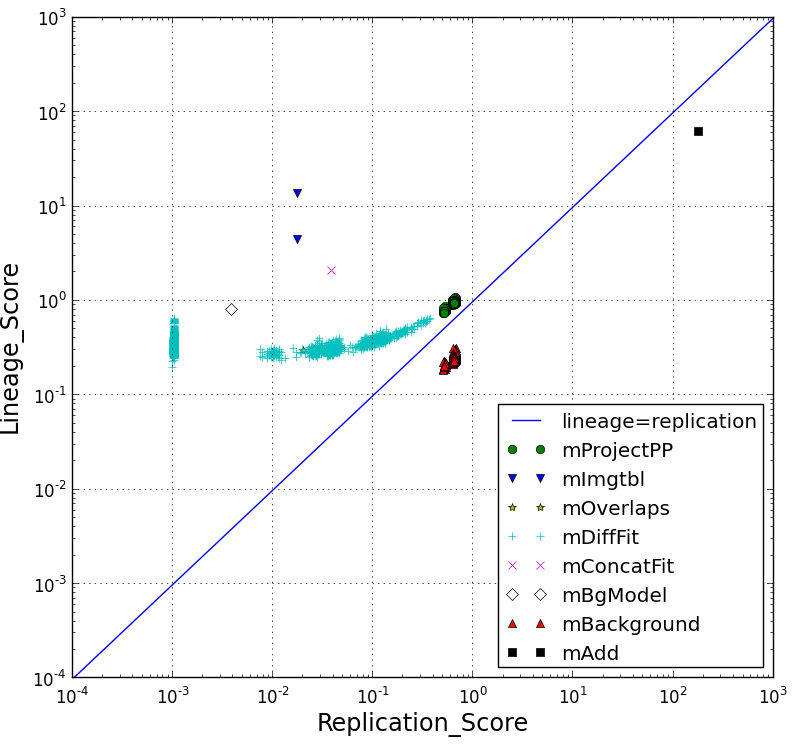
\includegraphics[width=70mm]{pictures/dist}
                \vspace{-10pt}
                \caption{Montage output files' positioning in a two dimensional space of replication score and re-execution score.
                \label{fig:montage-space}}
        \end{center}
\end{figure}

Figure~\ref{fig:montage-space} shows the position of all output files in the test case on a two dimensional space of re-execution and replication score
%\kylenote{cost? We never really define score. I dont mind calling it score but we should make sure that is clear earlier.} 
%\zhaonote{I put a Score definition before Equation 7. It is ``Score'' as it is the linear combination of the expected backup and recovery cost. So there should be ``Lineage Score'' and ``Replication Score'' for each file.}
calculated with Equation~\ref{EQ:combined}.
Each point shows a single output file from each Montage stage. The points in the upper left triangle are those where the replication score is lower than the re-execution store, 
while those in the lower right triangle are the files where the re-execution score is lower than the replication score.

\subsection{Recovery Performance}
To evaluate recovery time, we inject failures during job execution by causing a node to fail (fail-stop) at a specified application stage.
We inject failures in two specific stages, namely at the end of the mProject stage and the end of the mBackground stage,
in order to evaluate both single-stage recovery performance and multi-stage recovery (recursive recovery) performance.

\subsubsection{Single-Stage Recovery}
We first fail a node immediately after the mProject stage finishes, before the mImgtbl stage starts,
and evaluate the impact on the mImgtbl-1, mDiffFit, and mBackground stages, each of which
needs to access the output files of mProject.
When one of these files is not available, the system must recover that file through either re-execution (based on
lineage metadata) or by accessing a file replica (if the file replicated).

Figure~\ref{fig:montage-fail-mProjectPP} compares the time-to-solution of our three backup methods for those three
Montage stages.
We see that the adaptive and replication methods perform similarly in stages mImgtbl-1 and mDiffFit,
as the output files of these two stages are backed up via replication; both also perform better than the re-execution method.
The mBackground stage runs faster under the adaptive method than in the re-execution and replication method,
as all of its tasks benefit from the previously replicated mProject output files and all of its output files are backed up through the re-execution method as shown in Figure~\ref{fig:montage-space}.

\begin{figure}[ht]
        \begin{center}
                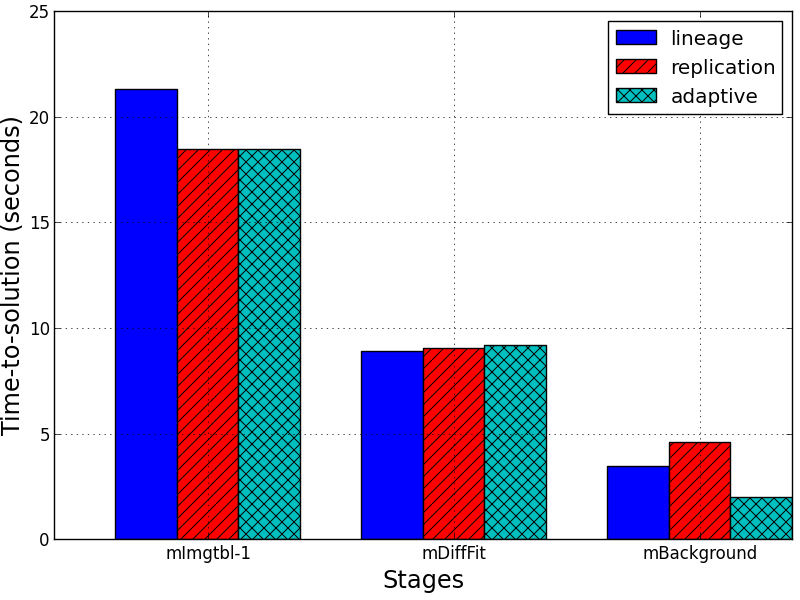
\includegraphics[width=75mm]{pictures/kill-mProjectPP}
                \vspace{-10pt}
                \caption{Recovery performance of mImgtbl, mDiffFit, and mBackground following a node failure that occurs after mProjectPP finishes and before mImgtbl starts.
                \label{fig:montage-fail-mProjectPP}}
        \end{center}
\end{figure}

\subsubsection{Multi-Stage Recovery}
We fail a node immediately after mBackground finishes, before mImgtbl-2 starts.
Both the mImgtbl-2 and mAdd stages need to access mBackground's output files.
However, in this case, a node failure results in the loss of output files from not only mBackground but also mProject---files
that we need in order to recover mBackground's outputs.
Thus, upon file unavailability, the system recovers the mBackground output file in multiple stages (recursively), as follows:
1) access to one mBackground output file fails;
2) the system tries to recover that mBackground output file by re-executing the task;
3) that task accesses an output of mProject;
4) that mProject output is unavailable;
5) the system recovers the missing mProject output.

\begin{figure}[h]
        \begin{center}
                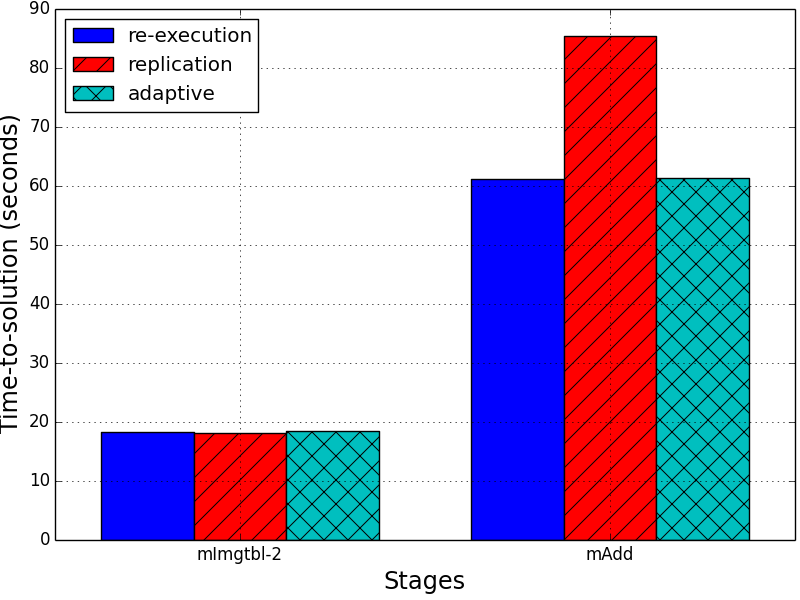
\includegraphics[width=75mm]{pictures/kill-mBack}
                \vspace{-10pt}
                \caption{Recovery performance of mImgtbl and mAdd due to a node failure occurred right after mBackground finishes and before mImgtbl starts
                \label{fig:montage-fail-mBackground}}
        \end{center}
\end{figure}

Figure~\ref{fig:montage-fail-mBackground} shows the time-to-solution comparison between the three replication methods. 
The adaptive method achieves similar performance with re-execution and replication method for mImgtbl-2. 
This indicates that recovery from re-execution recursively and backing up the mImgtbl-2 output file with the same method has identical performance to recovery using replication recursively and backing up mImgtbl-2 output files through replication. 
In fact, the adaptive method recovers the input files using re-execution for mBackground and using replication for mProject. The mImgtbl-2 output file is backed up through replication.
The adaptive method has significant performance advantages for the mAdd stage.
It again achieves recursive recovery via re-execution for mBackground and replication for mProject,
but chooses re-execution for mAdd, which in turn results in better time-to-solution.



\subsection{Impact of Optimization Weight}
\label{sec:Perf:Weight}
We use the output files of all stages of the Montage test case to evaluate how the optimization weight parameter $\alpha$ impacts the behavior of our adaptive method. %\kylenote{scheme or algorithm?} \katznote{In American English, a scheme always has negative connotations though I recognize that this is not the case in British (and apparently NZ English).} 
We fix all parameters in the system except $\alpha$, which we set variously to be 0.1, 0.5, and 0.9, indicating the user's concern with optimizing the failure-free run time.


Figure~\ref{fig:weight} shows the results. We see that as $\alpha$ increases, files move from the upper left triangle to the lower right triangle, with the result that the failure-free run time is shorter since more files are backed up through the re-execution method.
This result exactly matches the user's optimization goal of minimizing failure-free running time.

\begin{figure*}[ht]
	\begin{center}
		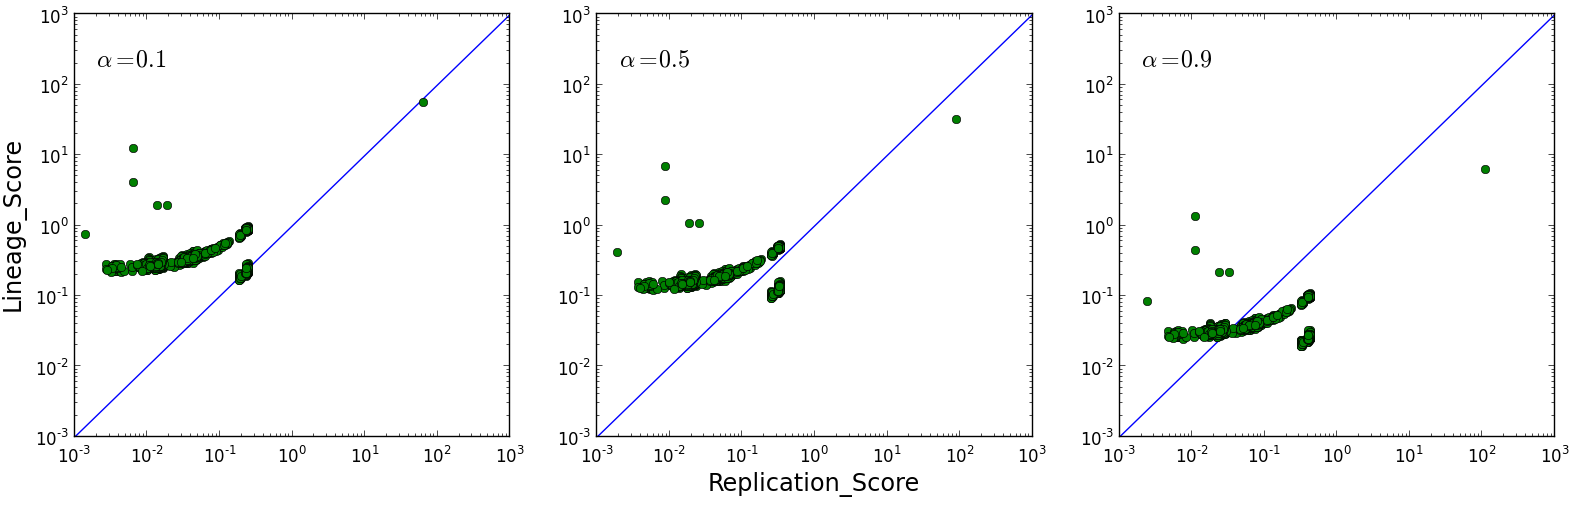
\includegraphics[width=160mm]{pictures/weight}
		\vspace{-10pt}
		\caption{Backup decisions at different optimization weights. Files in the upper left triangles are backed up through replication and files in the lower right triangles are backed up through re-execution.
		\label{fig:weight}}
  	\end{center}
\end{figure*}

\subsection{Impact of Failure Rate}
\label{sec:Perf:Failure}
The failure rate ($P$) of a computer system can be difficult to measure in practice.
For example, Amazon EC2 reports  system availability as a monthly uptime percentage~\cite{AWS-SLA}.
The Blue Gene/Q supercomputer's MTTF is reported as 1--7 days~\cite{Snir-resilience}, system-wide.
Given a customized allocation size
%\iannote{If we really knew the rate, that would be a simple arithmetic. Is the real issue that
%failure rates are not reported, not known, or are variable?} 
%\zhaonote{as the references show, it is hard to convert the numbers published to real use case, even though the number is directly failure rate, it means the overall system including compute nodes, network, storage.}
and hardware/software stack, it can be difficult for a user to convert these metrics to accurate MTTFs for a particular execution.

Surprisingly, the adaptive backup decisions remain the same under all five failure rate configurations of $P=\{\frac{1}{12}, \frac{1}{120},$ 
$\frac{1}{1200}, \frac{1}{12000}, \frac{1}{120000}\}$,
which implies that the failure rate is irrelevant to the adaptive backup decision, at least for this application.
The reason for this lack of sensitivity to $P$ becomes clear when we look at Equations~\ref{EQ:spatial} and \ref{EQ:temporal}.
We see that unless $P$ is quite large, data and metadata copy costs dominate,
%
%\katznote{should this be part of the previous paragraph?}
%\zhaonote{yes, done}
and the re-execution score and replication score have a simpler form than in Equations~\ref{EQ:spatial} and \ref{EQ:temporal}
%\iannote{What do you mean ``now"? And simpler than what? Why?}\zhaonote{simpler than Equation 5 and 6, since we eliminate the part with $P$ because $P$'s impact is limited}:
\begin{itemize}
  \item[] $S_{repl} = \alpha\frac{|y|}{B}(r-1) + (1-\alpha)\frac{|y|}{B} $
  \item[] $S_{line} = \alpha\frac{|M_y|}{B}(r-1) + (1-\alpha)T$
\end{itemize}

We also consider a second question, namely, how does the adaptive method respond to varying numbers of input files?
For example, in the case of {\em task 1} and {\em task 4} in Figure~\ref{fig:taxonomy}, which only differ in the number of input files, can the adaptive model determine that the output of {\em task 4} should be backed up through replication (since more input files indicate a larger chance of failure?)
The answer is yes.
Our computation of a task's time-to-solution $T$ includes three parts: input access (local or remote), computation time, and output to local RAM. If the computation and output phases take the same amount of time, more input files makes the input phase run longer, which is reflected in the measurement of $T$. The output of {\em task 4} thus has a higher recovery cost through re-execution than that of {\em task 1}; thus, the adaptive method is more likely to replicate the data.




\section{Related Work}
\label{sec:Related}
Researchers have investigated the optimum checkpointing interval~\cite{young1974first, daly2006higher}, coordinated checkpointing~\cite{chandy1985distributed}, and consistent checkpointing~\cite{elnozahy1992performance}, all for long-running tasks.  Common optimization goals in these approaches are minimizing: the time lost due to failures, failure-free running time (end-to-end time-to-solution of an application execution without any failure), and coordination overhead (e.g., minimizing the number of messages for all processes to reach a consistent checkpoint). 

Fault tolerant resilience models have been explored in small-scale applications for single-threaded applications on individual PCs~\cite{condor1988, libckpt1994}, large-scale distributed workflows~\cite{uncoordinated2010}, and parallel and HPC computing applications~\cite{mist1995, consistent1994,FTworkshop2009}, among others. In  general, most resilience approaches rely on some form of data replication, either explicitly via replicating intermediate files or implicitly via checkpointing application state.

Replication of intermediate files is often the easiest approach for building resilient applications. Such algorithms can be employed trivially by an execution framework or file system without requiring application modification. Replication techniques are also used to enhance scalability and performance. While specific goals may differ, the replication techniques applied are similar. A brief summary of replication techniques in distributed storage environments is presented in a survey~\cite{survey2012}. Replication techniques are often classified as either static or dynamic. In static configurations a set number of replicas and hosts are chosen at the start of the application lifecycle and are then used throughout execution. In a dynamic model these parameters are changed depending on access patterns, storage capacity, and bandwidth.  Dynamic models often employ a decentralized architecture in which replicas are distributed over a peer-to-peer network~\cite{chord} and decentralized decision mechanisms are used to place and access replicas. Replication techniques have been used for decades in distributed file systems such as the classic RAID~\cite{raid1988} and more recently HDFS~\cite{HDFS} and RAMCloud~\cite{ramcloud2010, ramcloud2014} to replicate files over a distributed collection of nodes. %\zhaonote{add one sentence}
The adaptive approach we present in this paper is more suitable for a different type of environment, with large numbers of diskless compute nodes.

Lineage strategies have been explored in scientific workflows~\cite{ramakrishnan09vgrads, calheiros13deadlines, Chimera2002} as well as in distributed computing framework such as Spark~\cite{RDD2012}. Most often, lineage in scientific workflows is motivated by the need to meet deadlines and therefore focuses on concurrent task replication. Thus, tasks are actively replicated on several nodes concurrently and the first result is taken. For example, in the VGrADS project~\cite{ramakrishnan09vgrads}, tasks are selectively replicated based on resource reliability and application performance models. Similar techniques are used in volunteer computing projects~\cite{boinc04} to establish consensus among several potentially untrusted sources. Spark, a data processing engine designed for processing Hadoop data, analyzes a task's \emph{lineage graph}---the operations used to build it---in order to reexecute entire tasks without requiring replication. This approach is particularly advantageous in the Spark context as individual tasks are short (50-200~ms) stream-based computations. %\zhaonote{add one sentence}
For many-task applications, run time and I/O amount can be highly irregular, so no single approach will always be the best solution.

Replication strategies have also been used to compute in the presence of faults, such as in algorithm-based fault tolerance (ABFT)~\cite{abft}, where checksums are used to limit the memory used to replicate.  Later work~\cite{turmon1, turmon2, gunnels} introduced the idea of using the checksums to detect faults, then using a lineage-like reexecution at various levels, from a function call, to an iteration within a function, to backup.

Checkpointing represents a more complex model for resilience in which copies of application state are made during execution and these copies enable applications to be reexecuted from checkpointed state. Checkpointing often requires intimate application knowledge to accurately capture process state and novel techniques to reduce storage overhead. This is important, because in large systems with thousands of processors, checkpoint data alone may exceed tens of terabytes~\cite{diskless2010}. For this reason, many different checkpointing approaches have been proposed. In general, approaches can be categorized as either application-, user-, or kernel-level. Application-level approaches are generally one-off implementations, highly optimized based on low-level application knowledge; while highly efficient, development is often expensive.
User- and kernel-level checkpointing enable applications to be checkpointed (periodically) during execution without requiring application modifications. In these models, users are often only minimally aware (in some cases they can provide `hints') of the checkpointing process as the underlying system captures complete application state to reexecute the applications. User level applications include Condor~\cite{condor1988} and libckpt~\cite{libckpt1994}. Kernel-level checkpointing is implemented at the operating system, common examples include Distributed MultiThreaded Checkpointing~\cite{dmtcp2009} and Berkeley Lab Checkpoint/Restart~\cite{blcr2006}. Checkpointing-based approaches have also been used to create resilient distributed programming runtimes such as MPICH-V~\cite{bosilca02mpichv} and rMPI~\cite{ferreira2011rmpi}.
There are other checkpointing research directions as well.
Optimum checkpointing interval~\cite{young1974first, daly2006higher} minimizes the lost work in case of a failure.
The consistent checkpointing~\cite{elnozahy1992performance, chandy1985distributed} synchronizes the checkpointed states of each individual process.
Checkpointing is typically used on long running tasks, while the tasks in our research are small tasks which can be seen as a natural partitioning of long running task. The long running parallel task abstraction also requires the processes to coordinate upon failure to reach consensus then all processes roll back to the coordinated checkpoint. This is not the case for small task abstraction. The whole execution is usually not halted or rolled back in a collective way, rather the execution continues when failures present, and the recovery decision is making by individual task rather than overall application.
 
In most cases both replication and checkpointing use stable (often distributed) file system storage for replicas, since these systems are resistant to processor failure. Researchers have investigated the use of disk in RAMCloud~\cite{ramcloud2011},  diskless~\cite{diskless1998, zhen04}, and in memory replicas as a means to reduce the I/O overhead of storing replicas on disk. Others have explored SSDs~\cite{diskless2010} as a compromise between in-memory and  disk-based approaches. These models use a number of techniques to avoid the bottlenecks seen with disk-based checkpointing techniques. Other optimizations including encoding techniques, such as erasure encoding~\cite{star2008, erasure2009}, have also been applied to reduce data storage requirements.


While these approaches to fault tolerance have been successfully applied in a number of domains they do not provide the same level of dynamism proposed in this work. Perhaps the most similar approaches are those employed in data location aware scheduling~\cite{diana2007,peris10location}. In these systems, the goal is to balance the tradeoff between the cost of transfer and the cost of compute. In such models, sophisticated schedulers determine if data should be moved to compute or vice versa. In many ways these comparisons are similar to the dynamic resiliency algorithms applied in our work; however, the approaches differ in that here we consider the latency within networks and the cost of storage, and then compare this to the cost of computing the files themselves. Moreover, our approach attempts to quantify the cost of reexecution of compute against the cost of storage, where the cost of reexecution is accurately known. In location aware scheduling approaches the cost of transfer and execution are generally estimated with the goal of reducing the overall execution time, irrespective of failure.  


\section{Conclusion and Future Work}
\label{sec:Con}
We have proposed a new method to fault-tolerant distributed computation suitable for the increasingly important class of parallel applications composed of small tasks linked by data flows when using parallel scripting frameworks with transient in-memory file systems. %\zhaonote{some more text in the previous sentence}
The core of our method is a mathematical model of backup and recovery costs, which we leverage to make runtime decisions about how and when to replicate data and metadata. This model, which permits online comparison of the cost of replicating data via either re-execution or access to replicas, takes as input only input file size, output file size, number of replicas, task time-to-solution, network bandwidth, and failure rate.
We implemented the model in a parallel scripting framework and presented performance results for an astronomy image processing application, Montage.
These results show that our adaptive method can recover from failure more efficiently in the case of failure than other methods, while introducing only 2.9\% overhead when there are no failures. We also investigated the sensitivity of our model to failure rate, a notoriously inaccurate parameter. We find that for our target application (and, we expect, for many other similar applications), backup decisions are relatively insensitive to failure rate in practice.

Our configurable model permits users to express their preferences regarding the relative weight to be given to re-execution vs.\ access to cached data as a recovery strategy,
and thus the time spent on data replication vs.\ metadata storage. Such preferences may be used to express, for example, the user's expected failure rates, their interest
in rapid failure-free execution, and/or their interest in limiting storage consumption for backups.

In future work, we plan to integrate this adaptive backup model with the Berkeley Data Analytics Stack, particularly with
the graph processing framework GraphX~\cite{graphx2014} and the memory centric storage system Tachyon~\cite{tachyon2014}.
We also plan to investigate a wider range of applications, explore extensions to incorporate other constraints such as limited backup storage,
and examine the use of asynchronous replication and hierarchical storage.

\section{Acknowledgments}
\katznote{anything else about funding sponsors to add?}
The AMPLab is supported in part by NSF CISE Expeditions Award CCF-1139158, LBNL Award 7076018, and DARPA XData Award FA8750-12-2-0331, and gifts from Amazon Web Services, Google, SAP,  The Thomas and Stacey Siebel Foundation, Adatao, Adobe, Apple, Inc., Blue Goji, Bosch, C3Energy, Cisco, Cray, Cloudera, EMC, Ericsson, Facebook, Guavus, Huawei, Intel, Microsoft, NetApp, Pivotal, Samsung, Splunk, Virdata, VMware, and Yahoo!. 
%\katznote{are all of these active supporters of work done in this paper?  If not, can we remove some of them? - not a big deal either way}
%\zhaonote{Unfortunately, all these sponsors have to be listed in the ack. }

The Berkeley Institute for Data Science (BIDS) is  supported by ... \katznote{todo.} 


Work by Katz was supported by the National
Science Foundation while working at the Foundation.  Any opinion, finding, and
conclusions or recommendations expressed in this material are those of the
author(s) and do not necessarily reflect the views of the National Science
Foundation.

\bibliographystyle{abbrv}
\bibliography{Resilience}


%\theendnotes

\end{document}







